\documentclass{article}
\usepackage[utf8]{inputenc}
\usepackage[russian]{babel}
\usepackage{amsmath,amsfonts,amsthm,amssymb}
\usepackage{tikz}
\usepackage{pgfplots}
\usepackage{float}
\usepackage{lipsum}
\usepackage{indentfirst}
\usepackage[a4paper, total={170mm,257mm},left=9mm, top=10mm, right=20]{geometry}

\begin{document}

\title{Расчётно-графическая работа по теме "Ряды Тейлора и Фурье"}
\date{\today}
\maketitle

\section{Введение}
В этой работе мы исследуем применение рядов Тейлора для аппроксимации функций и решения дифференциальных уравнений.

\section{Ряды Тейлора}

\subsection{Задача 1а}

Дан числовой ряд:

\begin{equation}
\sum_{n=1}^{\infty} \frac{(-1)^{n-1}}{\sqrt{3^n}*(2n-1)}.
\end{equation}

Этот ряд напоминает ряд Маклорена для функции $\arctan(x)$, который выглядит следующим образом:

\begin{equation}
\arctan(x) = \sum_{n=0}^{\infty} (-1)^n \frac{x^{2n+1}}{2n+1}.
\end{equation}

При замене $x$ на $1/\sqrt{3}$ в ряде для $\arctan(x)$ мы получим исходный числовой ряд. Следовательно, сумма числового ряда равна $\arctan(1/\sqrt{3}) = \pi/6$.

\subsection{Задача 1б}

Требуется найти первообразную функции $f(x) = \sin(x)/x$ в виде ряда Маклорена. Разложим $\sin(x)$ в ряд Маклорена:

\begin{equation}
\sin(x) = \sum_{n=0}^{\infty} \frac{(-1)^n x^{2n+1}}{(2n+1)!}.
\end{equation}

Теперь можем представить функцию $f(x)$ в виде степенного ряда:

\begin{equation}
f(x) = \sum_{n=0}^{\infty} \frac{(-1)^n x^{2n}}{(2n+1)!}.
\end{equation}

Интегрируем это выражение для нахождения первообразной:

\begin{equation}
\int f(x) dx = \sum_{n=0}^{\infty} \frac{(-1)^n x^{2n+1}}{(2n+1)(2n+1)!} + C,
\end{equation}

где $C$ - константа интегрирования.

\newpage
\subsection{Задача 1в}

Рассмотрим дифференциальное уравнение и начальные условия:
\begin{equation*}
\begin{cases}
   y' = \frac{x}{\sqrt{y}} + 2 \\
   y(0) = 1 \\
\end{cases}
\end{equation*}
Допустим, что решение можно представить в виде степенного ряда:
\begin{equation*}
y(x) = y(0) + y'(0)x + \frac{y''(0)}{2!}x^2 + \frac{y'''(0)}{3!}x^3 + \frac{y''''(0)}{4!}x^4 + \ldots
\end{equation*}
Согласно заданным условиям, вычисляем первые четыре производные в точке x=0:
\begin{align*}
y(0) &= 1, \\
y'(0) &= 2, \\
y''(0) &= \frac{1}{2}, \\
y'''(0) &= \frac{1}{4}, \\
\end{align*}
Чтобы вычислить четвертую производную в точке x=0, продолжаем процесс дифференцирования:
\begin{equation*}
y'''' = \frac{3}{8} y^{-5/2}
\end{equation*}

Подставляем y(0) = 1 и получаем $y''''(0) = 
\frac{3}{8}$.

Тогда, приближённое решение до четвертого порядка будет:
\begin{equation*}
y(x) \approx y(0) + y'(0)x + \frac{y''(0)}{2!}x^2 + \frac{y'''(0)}{3!}x^3 + \frac{y''''(0)}{4!}x^4 = 1 + 2x + \frac{1}{2}x^2 + \frac{1}{24}x^3 + \frac{1}{192}x^4
\end{equation*}

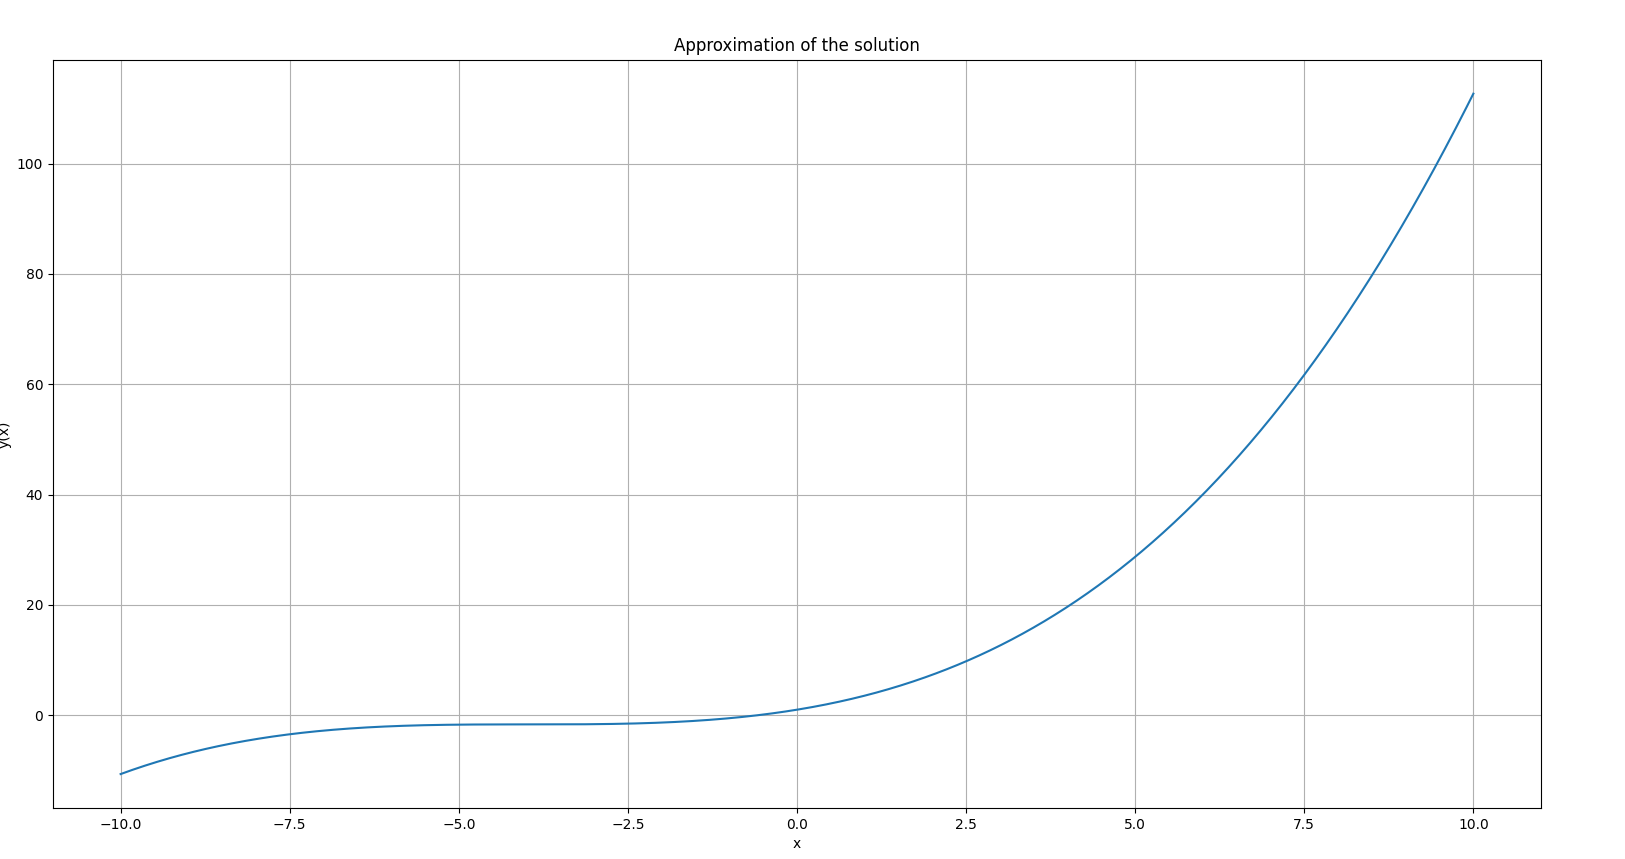
\includegraphics[width=\textwidth,height=10cm,keepaspectratio]{Approx.png}

\end{document}
